\documentclass[aspectratio=1610]{beamer}
\usepackage[T1]{fontenc}
\usetheme{wildcat}

\usepackage{amsmath,amssymb,amsfonts}
\usepackage{booktabs}
\usepackage{relsize}
\usepackage[export]{adjustbox}
\usepackage{listings}
\lstset{%
  basicstyle=\small\ttfamily\color{wcprimary},
  language=[LaTeX]{TeX},
  backgroundcolor=\color{white},
  xleftmargin=0.1cm,
  rulecolor=\color{wcprimary},
  frame=single,
  aboveskip=7pt,
  %framesep=8pt,
  %framerule=1pt
}

\usepackage[style=verbose,backend=biber]{biblatex}
\addbibresource{references.bib}
\let\oldfootnotesize\footnotesize
\renewcommand*{\footnotesize}{\oldfootnotesize\tiny}

\def\mathdefault#1{#1}
\everymath=\expandafter{\the\everymath\displaystyle}

\title{\LaTeX{} 101 \\ {\small ME 800 Seminar}}
\date{April 15, 2025}
\author{Jeremy Roberts}

\begin{document}

\begin{frame}
  \titlepage
\end{frame}

\section{Standalone \LaTeX{} Documents}

%%%%%%%%%%%%%%%%%%%%%%%%%%%%%%%%%%%%%%%%%%%%%%%%%%%%%%%%%%%%%%%%%%%%%%%%%%%%%%%
\begin{frame}[fragile]{A Barebones Document}
  \begin{columns}[T]

    \column{0.50\textwidth}

      \lstinputlisting[]{example_article.tex}

      \vspace{0.25cm}

      \raggedleft {\it Shown above is the \textcolor{wcprimary}{plain-text, LaTeX source}.  At right is
      the compiled PDF, and below, a zoomed view of the PDF.}

      \vspace{0.25cm}

      
\includegraphics[width=1.01\textwidth, trim={5cm 22cm 8cm 3cm},
                       clip, frame]{example_article.pdf}


    \column{0.50\textwidth}
      %  trim={<left> <lower> <right> <upper>}

      
\includegraphics[width=0.9\textwidth, frame]{example_article.pdf}

  \end{columns}
\end{frame}

%%%%%%%%%%%%%%%%%%%%%%%%%%%%%%%%%%%%%%%%%%%%%%%%%%%%%%%%%%%%%%%%%%%%%%%%%%%%%%%
\begin{frame}[fragile]{The Preamble and some {\it Lorem Ipsum}}
  \begin{columns}[T]

    \column{0.50\textwidth}

      \lstinputlisting{example_lorem.tex}

      \raggedleft {\it The default fonts come from the Computer Modern family invented by
      the inventor of \TeX{}, Donald Knuth.}

    \column{0.50\textwidth}
      %  trim={<left> <lower> <right> <upper>}

      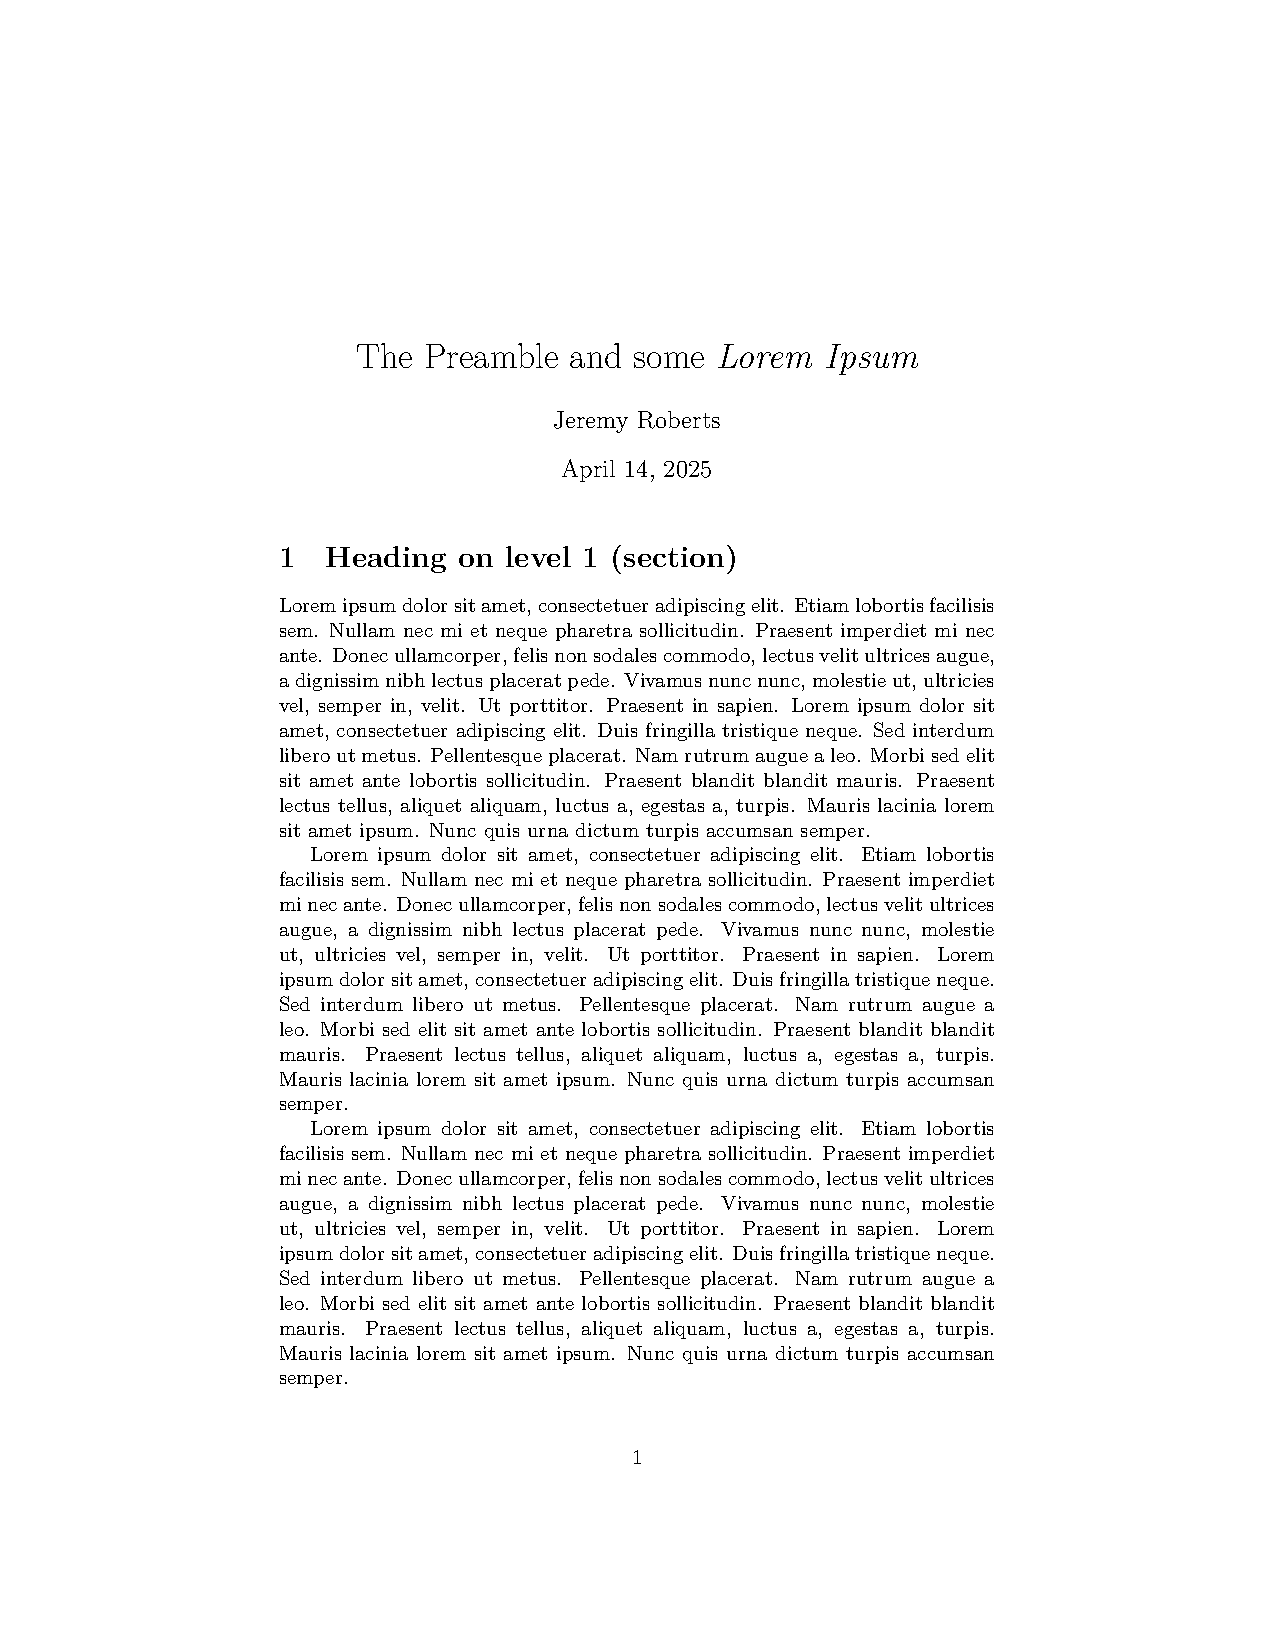
\includegraphics[width=0.9\textwidth, frame]{example_lorem.pdf}

  \end{columns}
\end{frame}


%%%%%%%%%%%%%%%%%%%%%%%%%%%%%%%%%%%%%%%%%%%%%%%%%%%%%%%%%%%%%%%%%%%%%%%%%%%%%%%
\begin{frame}[fragile]{Tweaking Formats}
  \begin{columns}[T]

    \column{0.50\textwidth}

      \lstinputlisting{example_formatting.tex}

    \column{0.50\textwidth}
      %  trim={<left> <lower> <right> <upper>}

      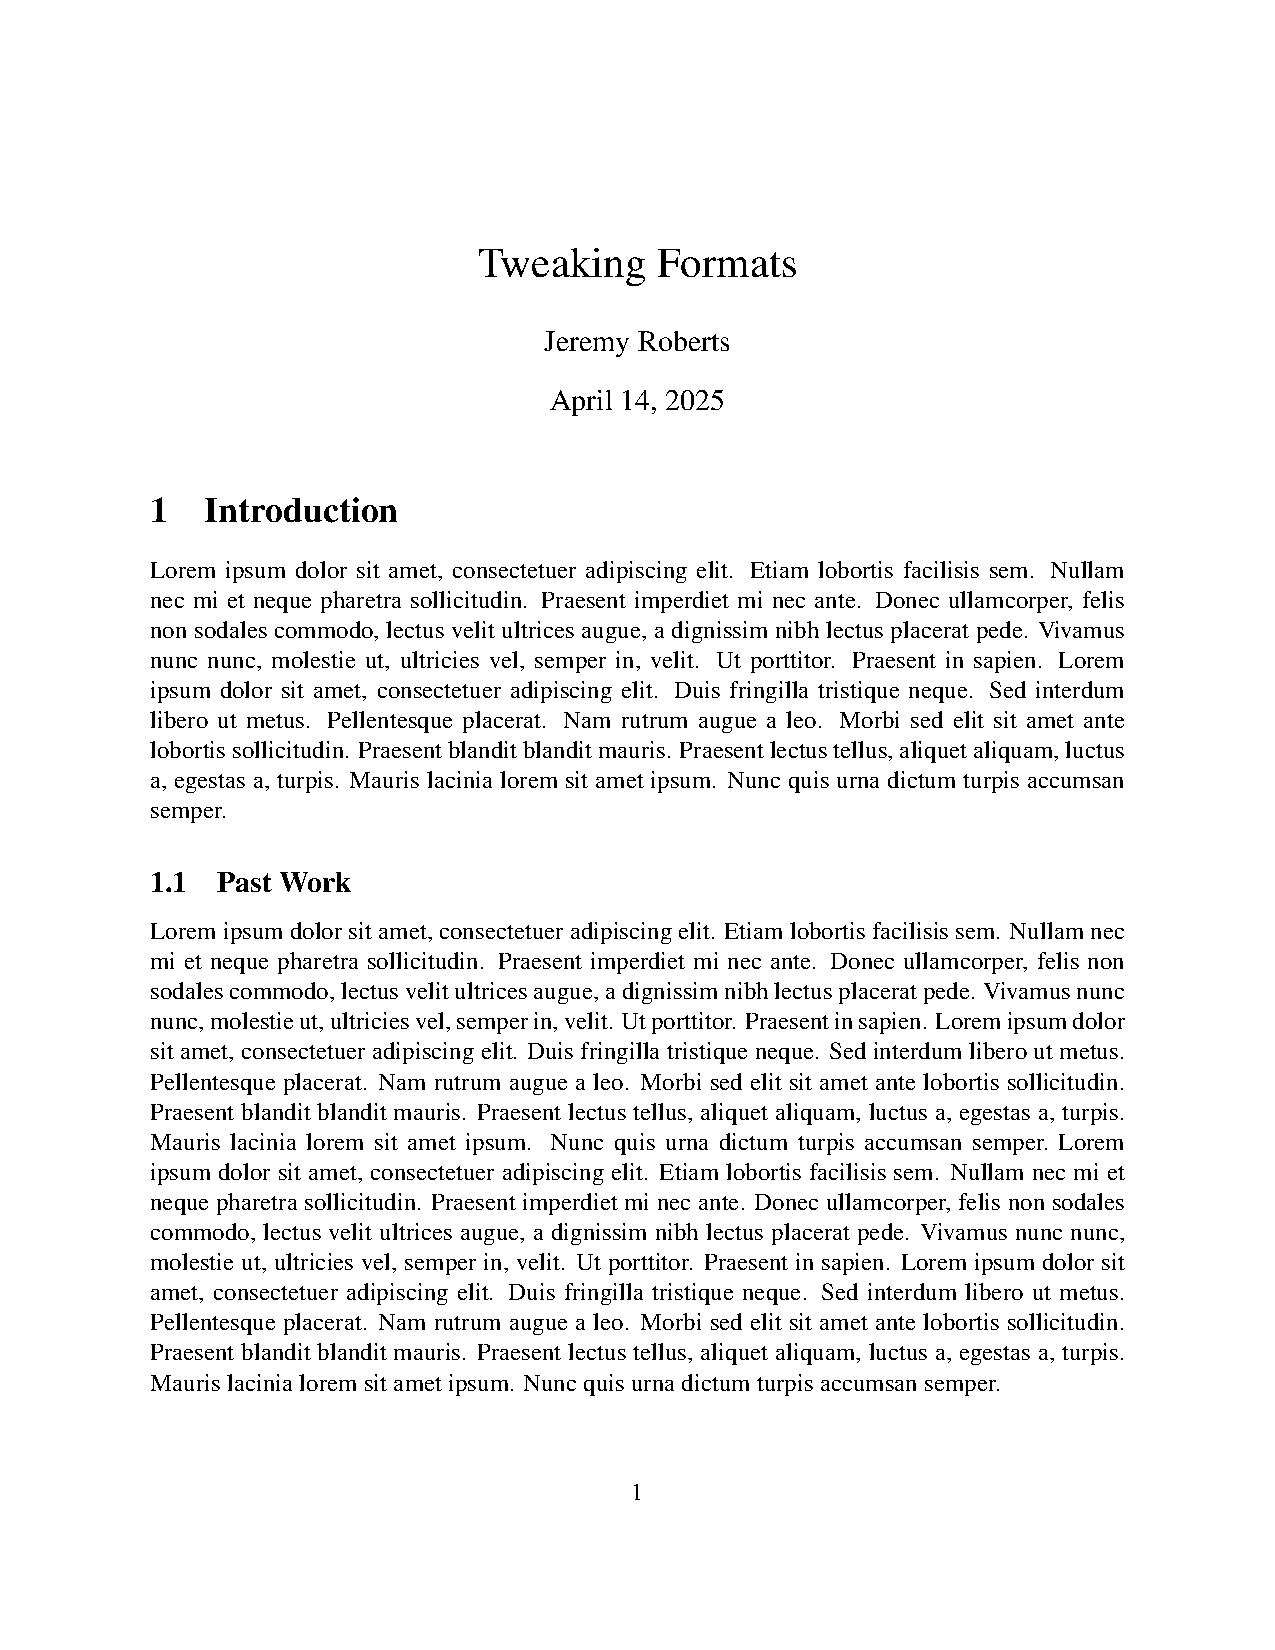
\includegraphics[width=0.9\textwidth, frame]{example_formatting.pdf}

  \end{columns}
\end{frame}

%%%%%%%%%%%%%%%%%%%%%%%%%%%%%%%%%%%%%%%%%%%%%%%%%%%%%%%%%%%%%%%%%%%%%%%%%%%%%%%
\begin{frame}[fragile]{A Journal Article}
  \begin{columns}[T]

    \column{0.50\textwidth}

      \vspace{-5pt}

      \lstinputlisting[basicstyle=\footnotesize\ttfamily\color{wcprimary}]{example_journal.tex}

      \raggedleft {\it Many templates and classes available!}

    \column{0.50\textwidth}

      %  trim={<left> <lower> <right> <upper>}
      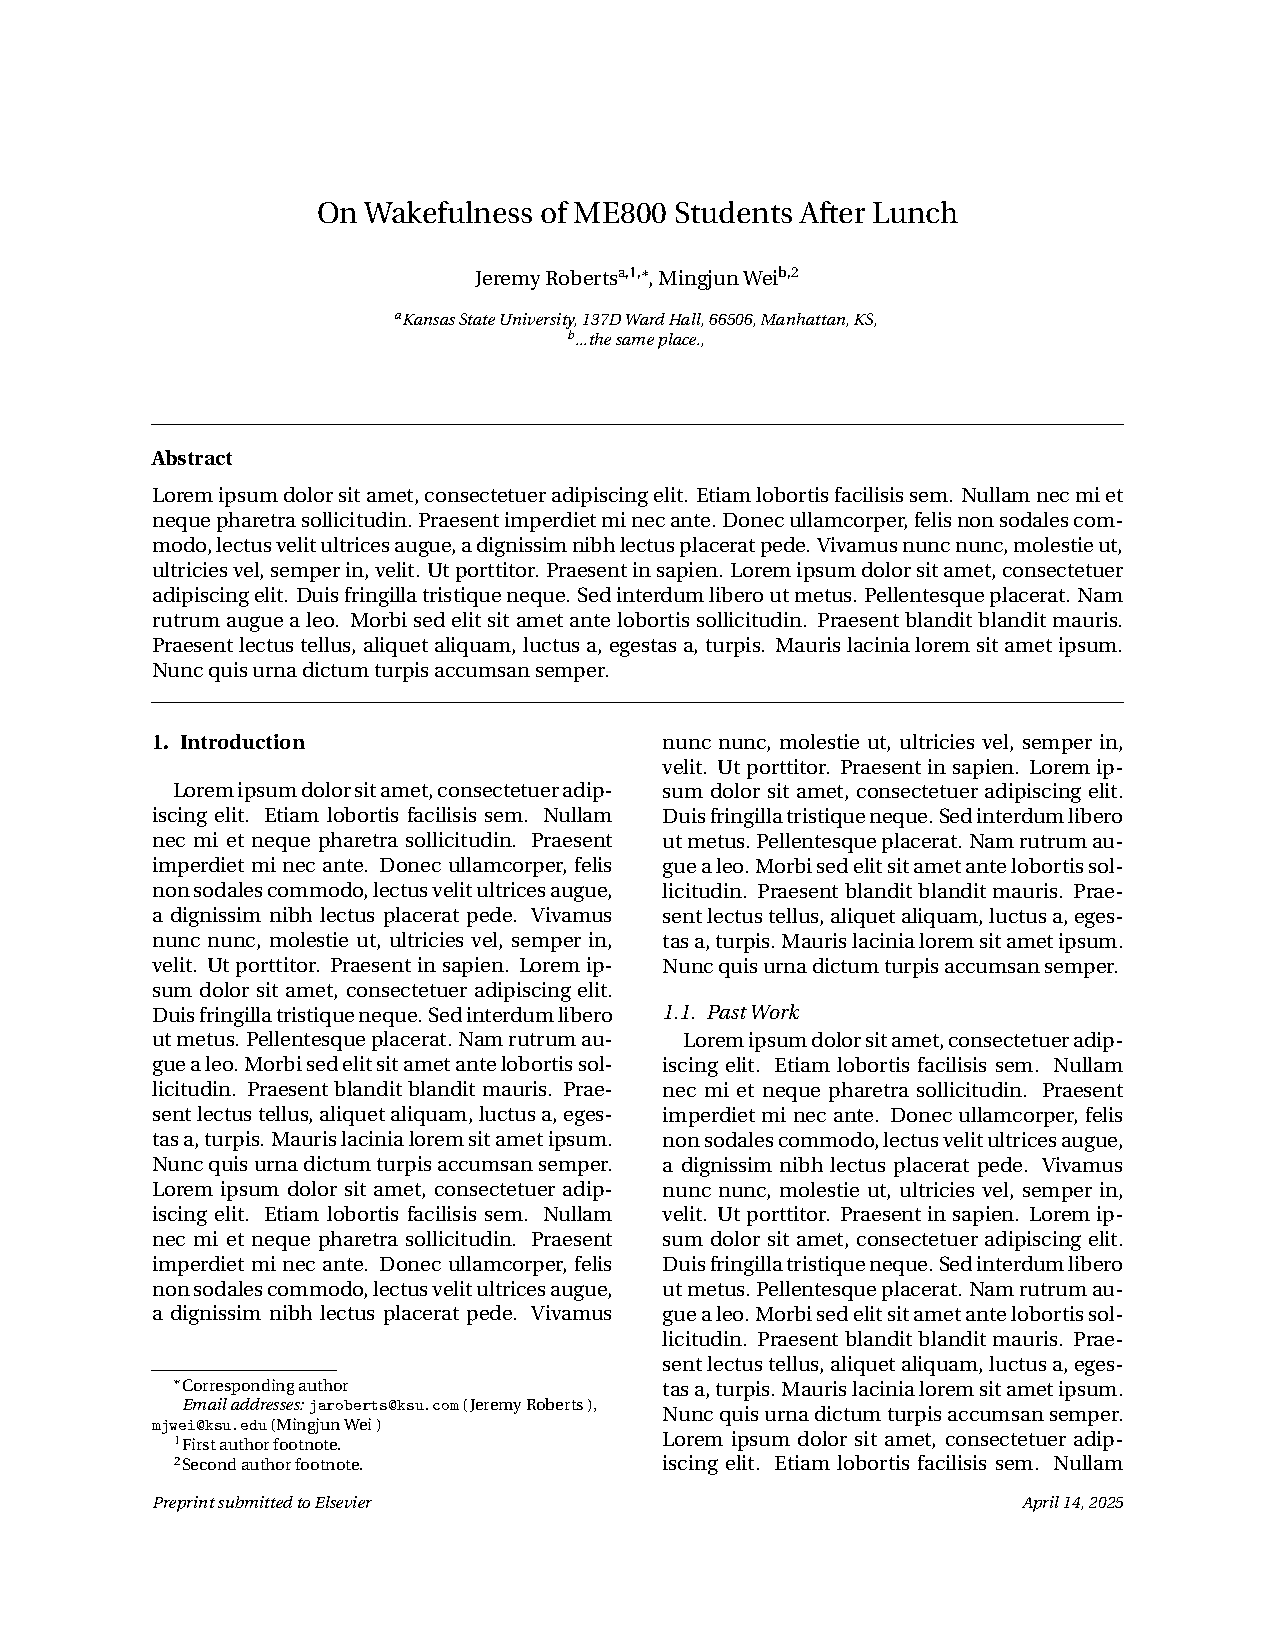
\includegraphics[width=0.9\textwidth, frame]{example_journal.pdf}

  \end{columns}
\end{frame}

%%%%%%%%%%%%%%%%%%%%%%%%%%%%%%%%%%%%%%%%%%%%%%%%%%%%%%%%%%%%%%%%%%%%%%%%%%%%%%%
\begin{frame}[fragile]{Thesis Support}

  \begin{columns}[T]

    \column{0.55\textwidth}

      \begin{itemize}
      \item An official \LaTeX{} template is available for K-State theses and dissertations:\\
          \url{https://www.k-state.edu/grad/academics/etdr/template/}
      \item A video tutorial is available:\\
          \url{https://youtu.be/XyiD893gpR4}
      \item The template is also available on Overleaf!
      \end{itemize}

    \column{0.45\textwidth}

      
\includegraphics[width=0.99\textwidth, frame]{example_thesis.pdf}

  \end{columns}

\end{frame}


%%%%%%%%%%%%%%%%%%%%%%%%%%%%%%%%%%%%%%%%%%%%%%%%%%%%%%%%%%%%%%%%%%%%%%%%%%%%%%%
\section{Core \LaTeX{} Structures}

%%%%%%%%%%%%%%%%%%%%%%%%%%%%%%%%%%%%%%%%%%%%%%%%%%%%%%%%%%%%%%%%%%%%%%%%%%%%%%%
\begin{frame}[fragile]{Lists and Enumerations}
  \begin{columns}[T]

    \column{0.50\textwidth}

\begin{lstlisting}
Unumbered lists of items:
\begin{itemize}
   \item First level item
   \item First level item
   \begin{itemize}
     \item Second level item
     \item Second level item
   \end{itemize}
\end{itemize}

Numbered lists:
\begin{enumerate}
    \item Item one
    \item Item two
\end{enumerate}
\end{lstlisting}

    \column{0.50\textwidth}

 \vbox to .7\textheight{%
Unumbered lists of items:
\begin{itemize}
   \item First level item 1
   \item First level item 2
   \begin{itemize}
     \item Second level item 1
     \item Second level item 2
   \end{itemize}
\end{itemize}


Numbered lists:
\begin{enumerate}
    \item Item 1
    \item Item 2
\end{enumerate}



\raggedleft {\it Like with code, it helps
to use white space to improve readability
of \LaTeX{}.}
}
  \end{columns}

\end{frame}

\end{document}

